\chapter{Caracterización y resultados experimentales}
\label{chap:results}
\textit{}
\vfill
\minitoc
\newpage

\section{Experimentos sobre $ CdTe (001) $ y $ CdTe(001)/Ag $}
\label{sec:chap4-cdte}

La muestra $ CdTe(001)/Ag $ fue sometida a tres evaporaciones de Ag dentro de una Cámara de Ultra Alto Vacío 
\textit{(UHVC)} por medio de la técnica Deposición Física por Haz de Electrones \textit{(EBPVD)}, con el 
fin de entender la interfaz metal/semiconductor y sus propiedades, intentando simular el comportamiento de 
superficie conductora/metálica y bulto aislante/semiconductor, el cual esta presente en los aislantes 
topológicos. La deposición de un material sobre otro con diferente parámetro de red, causa tensión en la 
interfaz de los materiales, provocando un cambio en el diagrama de bandas del semiconductor.
En esta sección se discuten los espectros de \textit{RDS} a través de los procesos a los que se fue sometida 
la muestra, además de la caracterización de la misma por medio de Espectroscopia Raman para observar la 
interfaz y la tensión relativa, \textit{AFM} y \textit{NSOM} para observar la morfología de la superficie.

\subsection{Evolución de la deposición de Ag sobre $ CdTe (001) $}
\label{sec:chap4-cdte-rds}

$e^{{X}}$

\subsection{Espectroscopia Raman}
\label{sec:chap4-cdte-raman}

Para comenzar con el análisis de los espectros Raman, cabe recalcar que dependiendo de la simetría 
del material puede o no ser \textit{Raman Activo}, esto quiere decir que no todos los materiales 
presentaran una respuesta al ser estudiados. Un ejemplo es la plata \textit{(Ag)}, la cual por 
la simetría que presenta, es un material \textit{inactivo}, pero aun asi, tiene efectos sobre el 
espectro cuando se presenta como una película delgada, como el presentar \textit{fluorescencia}, 
que es la propiedad de absorber la energía proveniente del espectro electromagnético y emitirla 
con una frecuencia diferente. Además que Ag siempre se comporta como un potenciador de la respuesta 
óptica, por lo que debemos trabajar con baja potencia para poder obtener una respuesta del material 
y no solo fluorescencia.

\begin{figure}[h!]
    \centering
    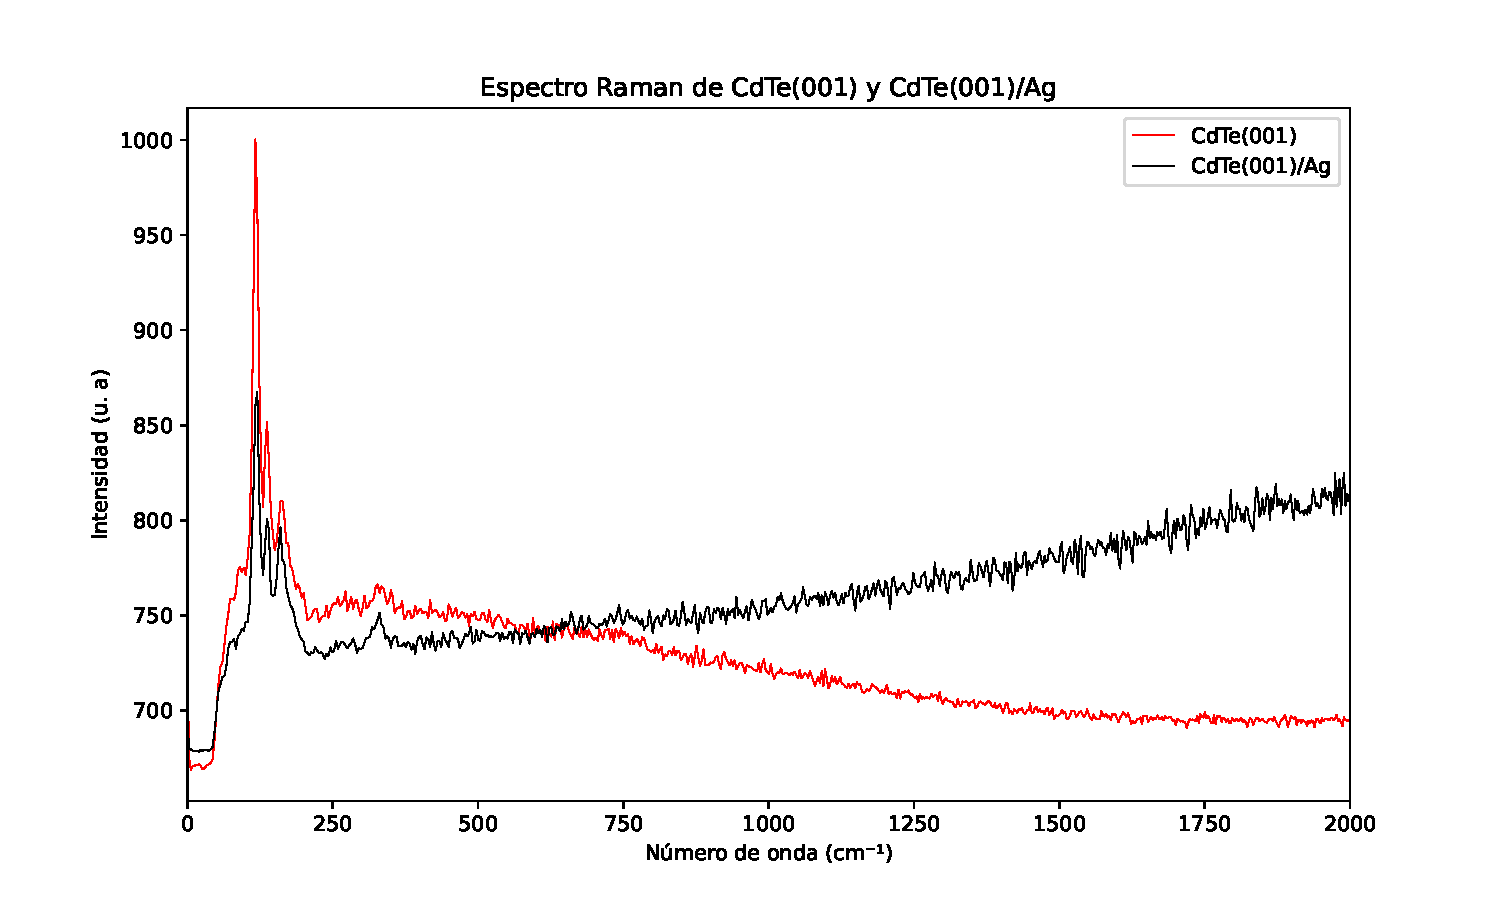
\includegraphics[width=0.7\textwidth]{figures/chap4/raman-CdTeAg-all.pdf}
        \caption{Espectro Raman obtenido para la muestra CdTe(001) y CdTe(001)/Ag, donde se
        puede notar la presencia de la fluorescencia causada por Ag mientras mas nos 
        acercamos al final del espectro.}
    \label{fig:raman-cdte-all}
\end{figure}

El fenómeno que nos interesa observar esta dentro del rango de 0-250 $cm^{-1}$, donde podemos observar 
los principales picos de la muestra. Debido a la tensión a la que esta sometida la muestra 
CdTe(001)/Ag, por la diferencia de parámetro de red entre ambos materiales existen dos fenómenos 
que vemos en el siguiente espectro Raman.

\begin{figure}[h!]
    \centering
    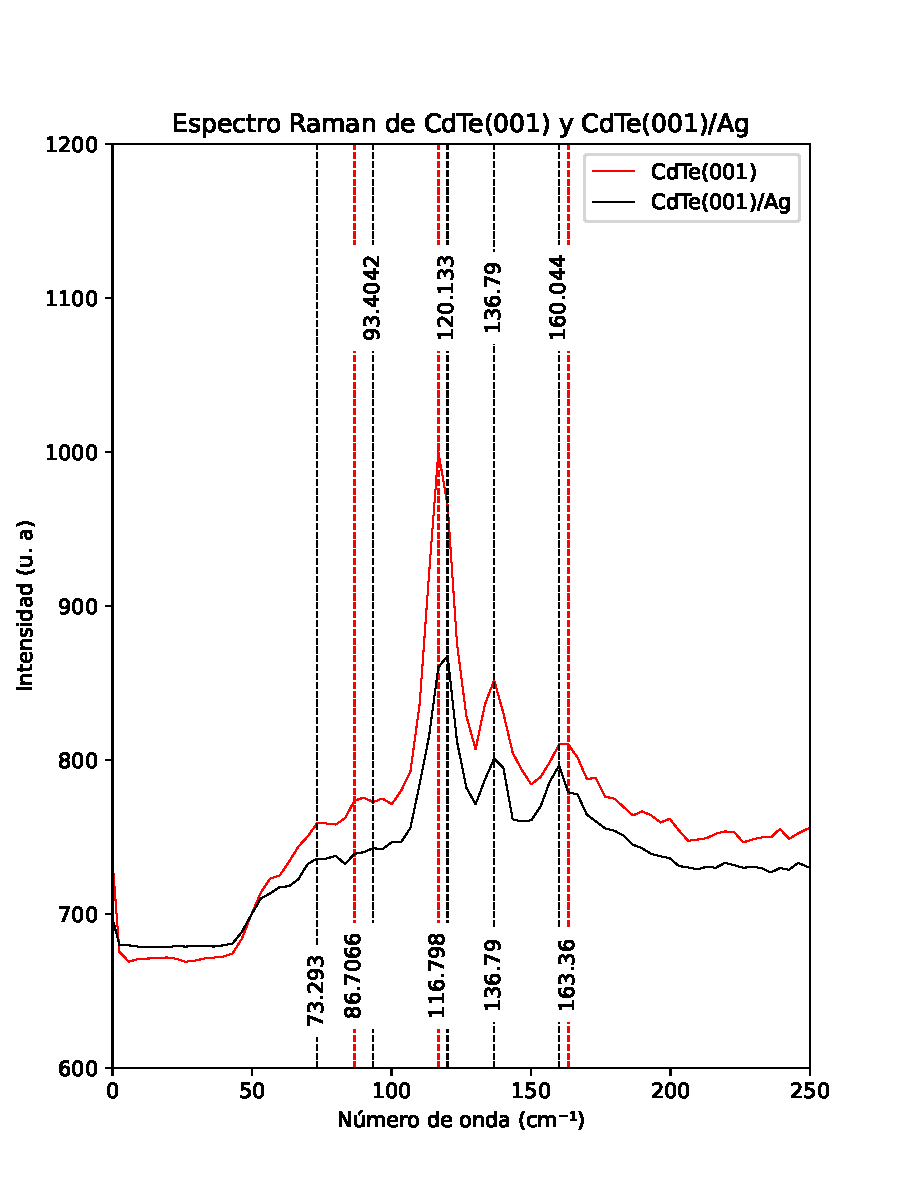
\includegraphics[width=0.5\textwidth]{figures/chap4/raman-CdTeAg-250.pdf}
        \caption{Espectro Raman obtenido para la muestra CdTe(001) y CdTe(001)/Ag, uno de ellos 
        fue trasladado para observarlo mejor.}
    \label{fig:raman-cdte-all}
\end{figure}

En este espectro, podemos apreciar el corrimiento de algunos picos, lo cual indica la presencia de 
estrés o tensión. En la Tabla ?, se condensa la información importante, que es la posición y el 
FWHM, que nos da una idea sobre la cristalinidad de la interfaz.

\subsection{AFM y NSOM}
\label{sec:ch4-cdte-afm-nsom}
Para la medición de estas dos técnicas se observaron dos zonas diferentes, las cuales se muestran en la 
Figura \ref{fig:afm-zones}.

\begin{figure}[h!]
    \centering
    \begin{subfigure}[b]{0.45\textwidth}
        \centering
        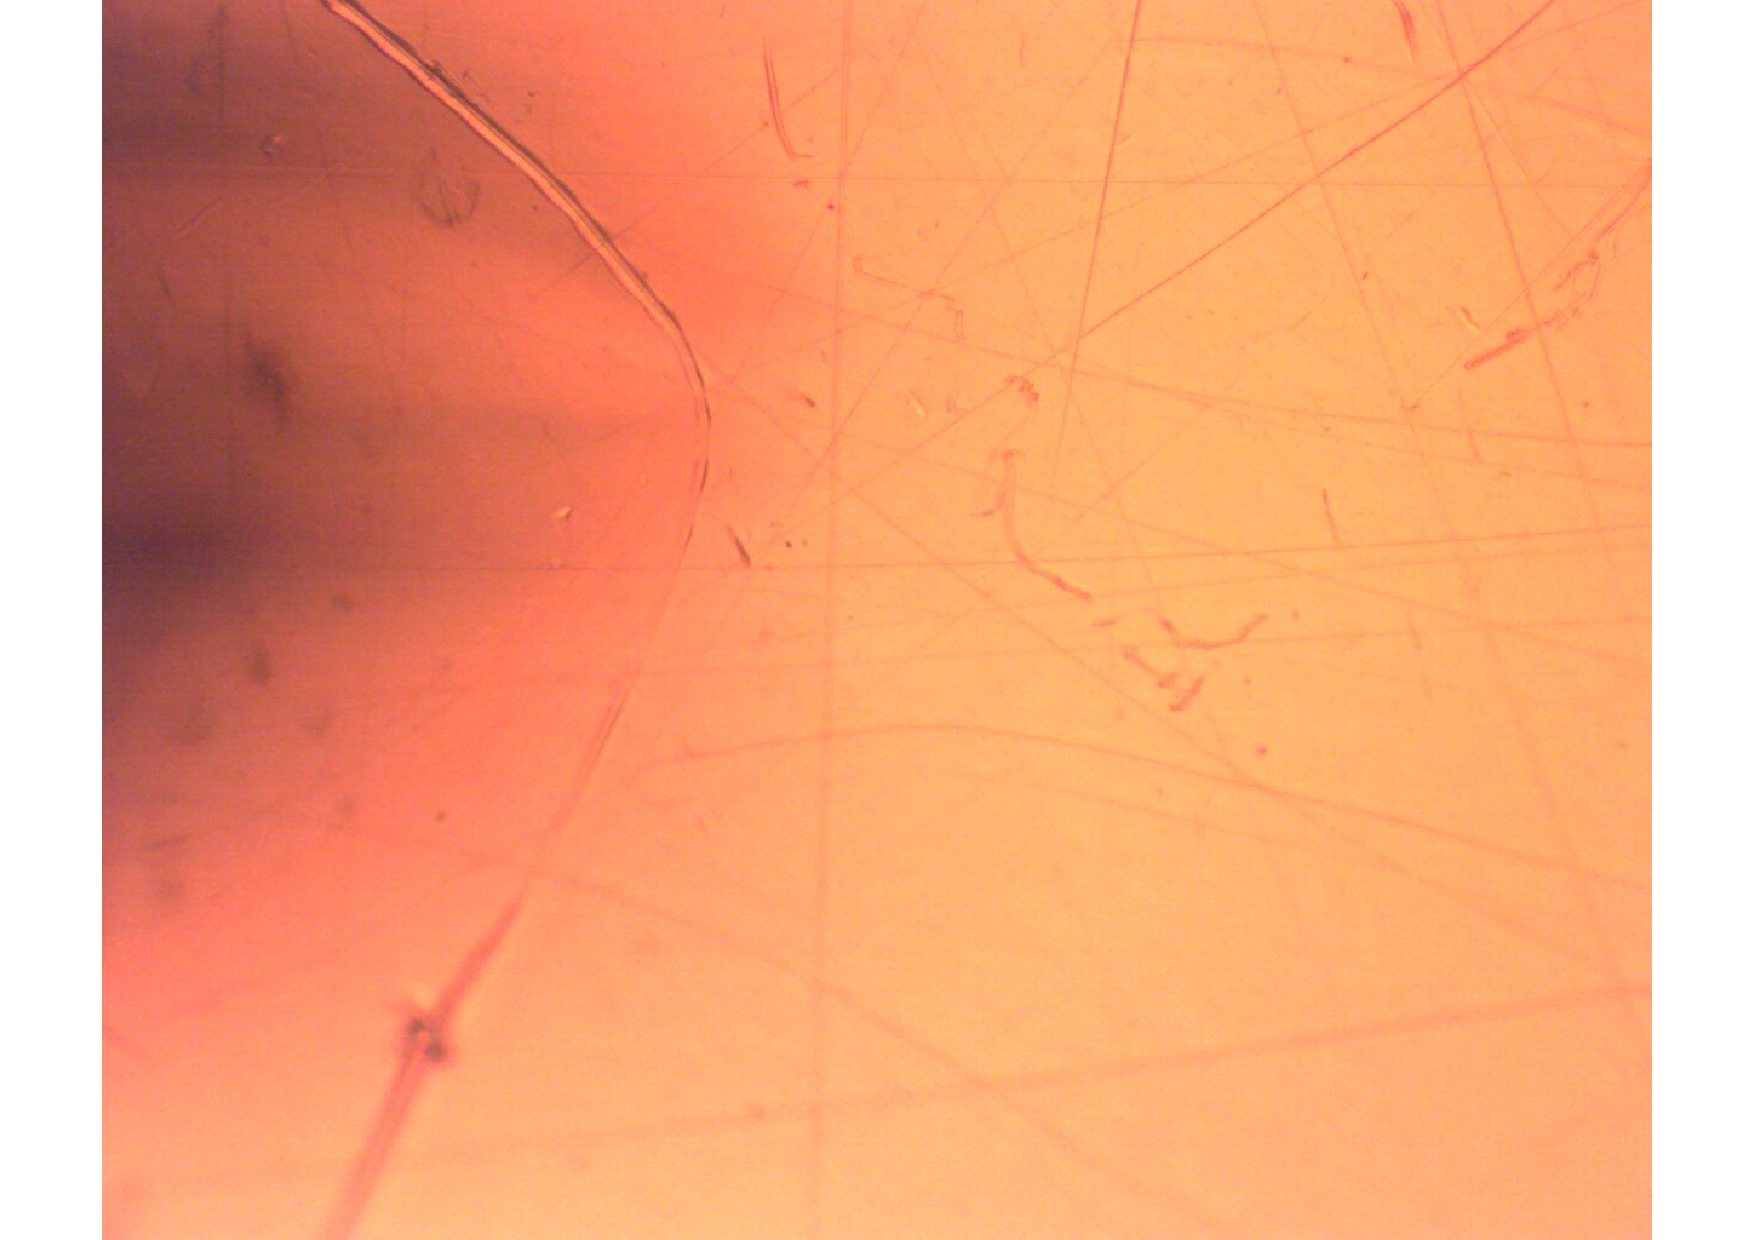
\includegraphics[width = 1\textwidth]{figures/chap4/CdTe_Ag_Zona1_10X.pdf}
        \subcaption{Zona 1 donde se realizo la medición de AFM y NSOM.}
    \end{subfigure}\hfill
    \begin{subfigure}[b]{0.42\textwidth}
        \centering
        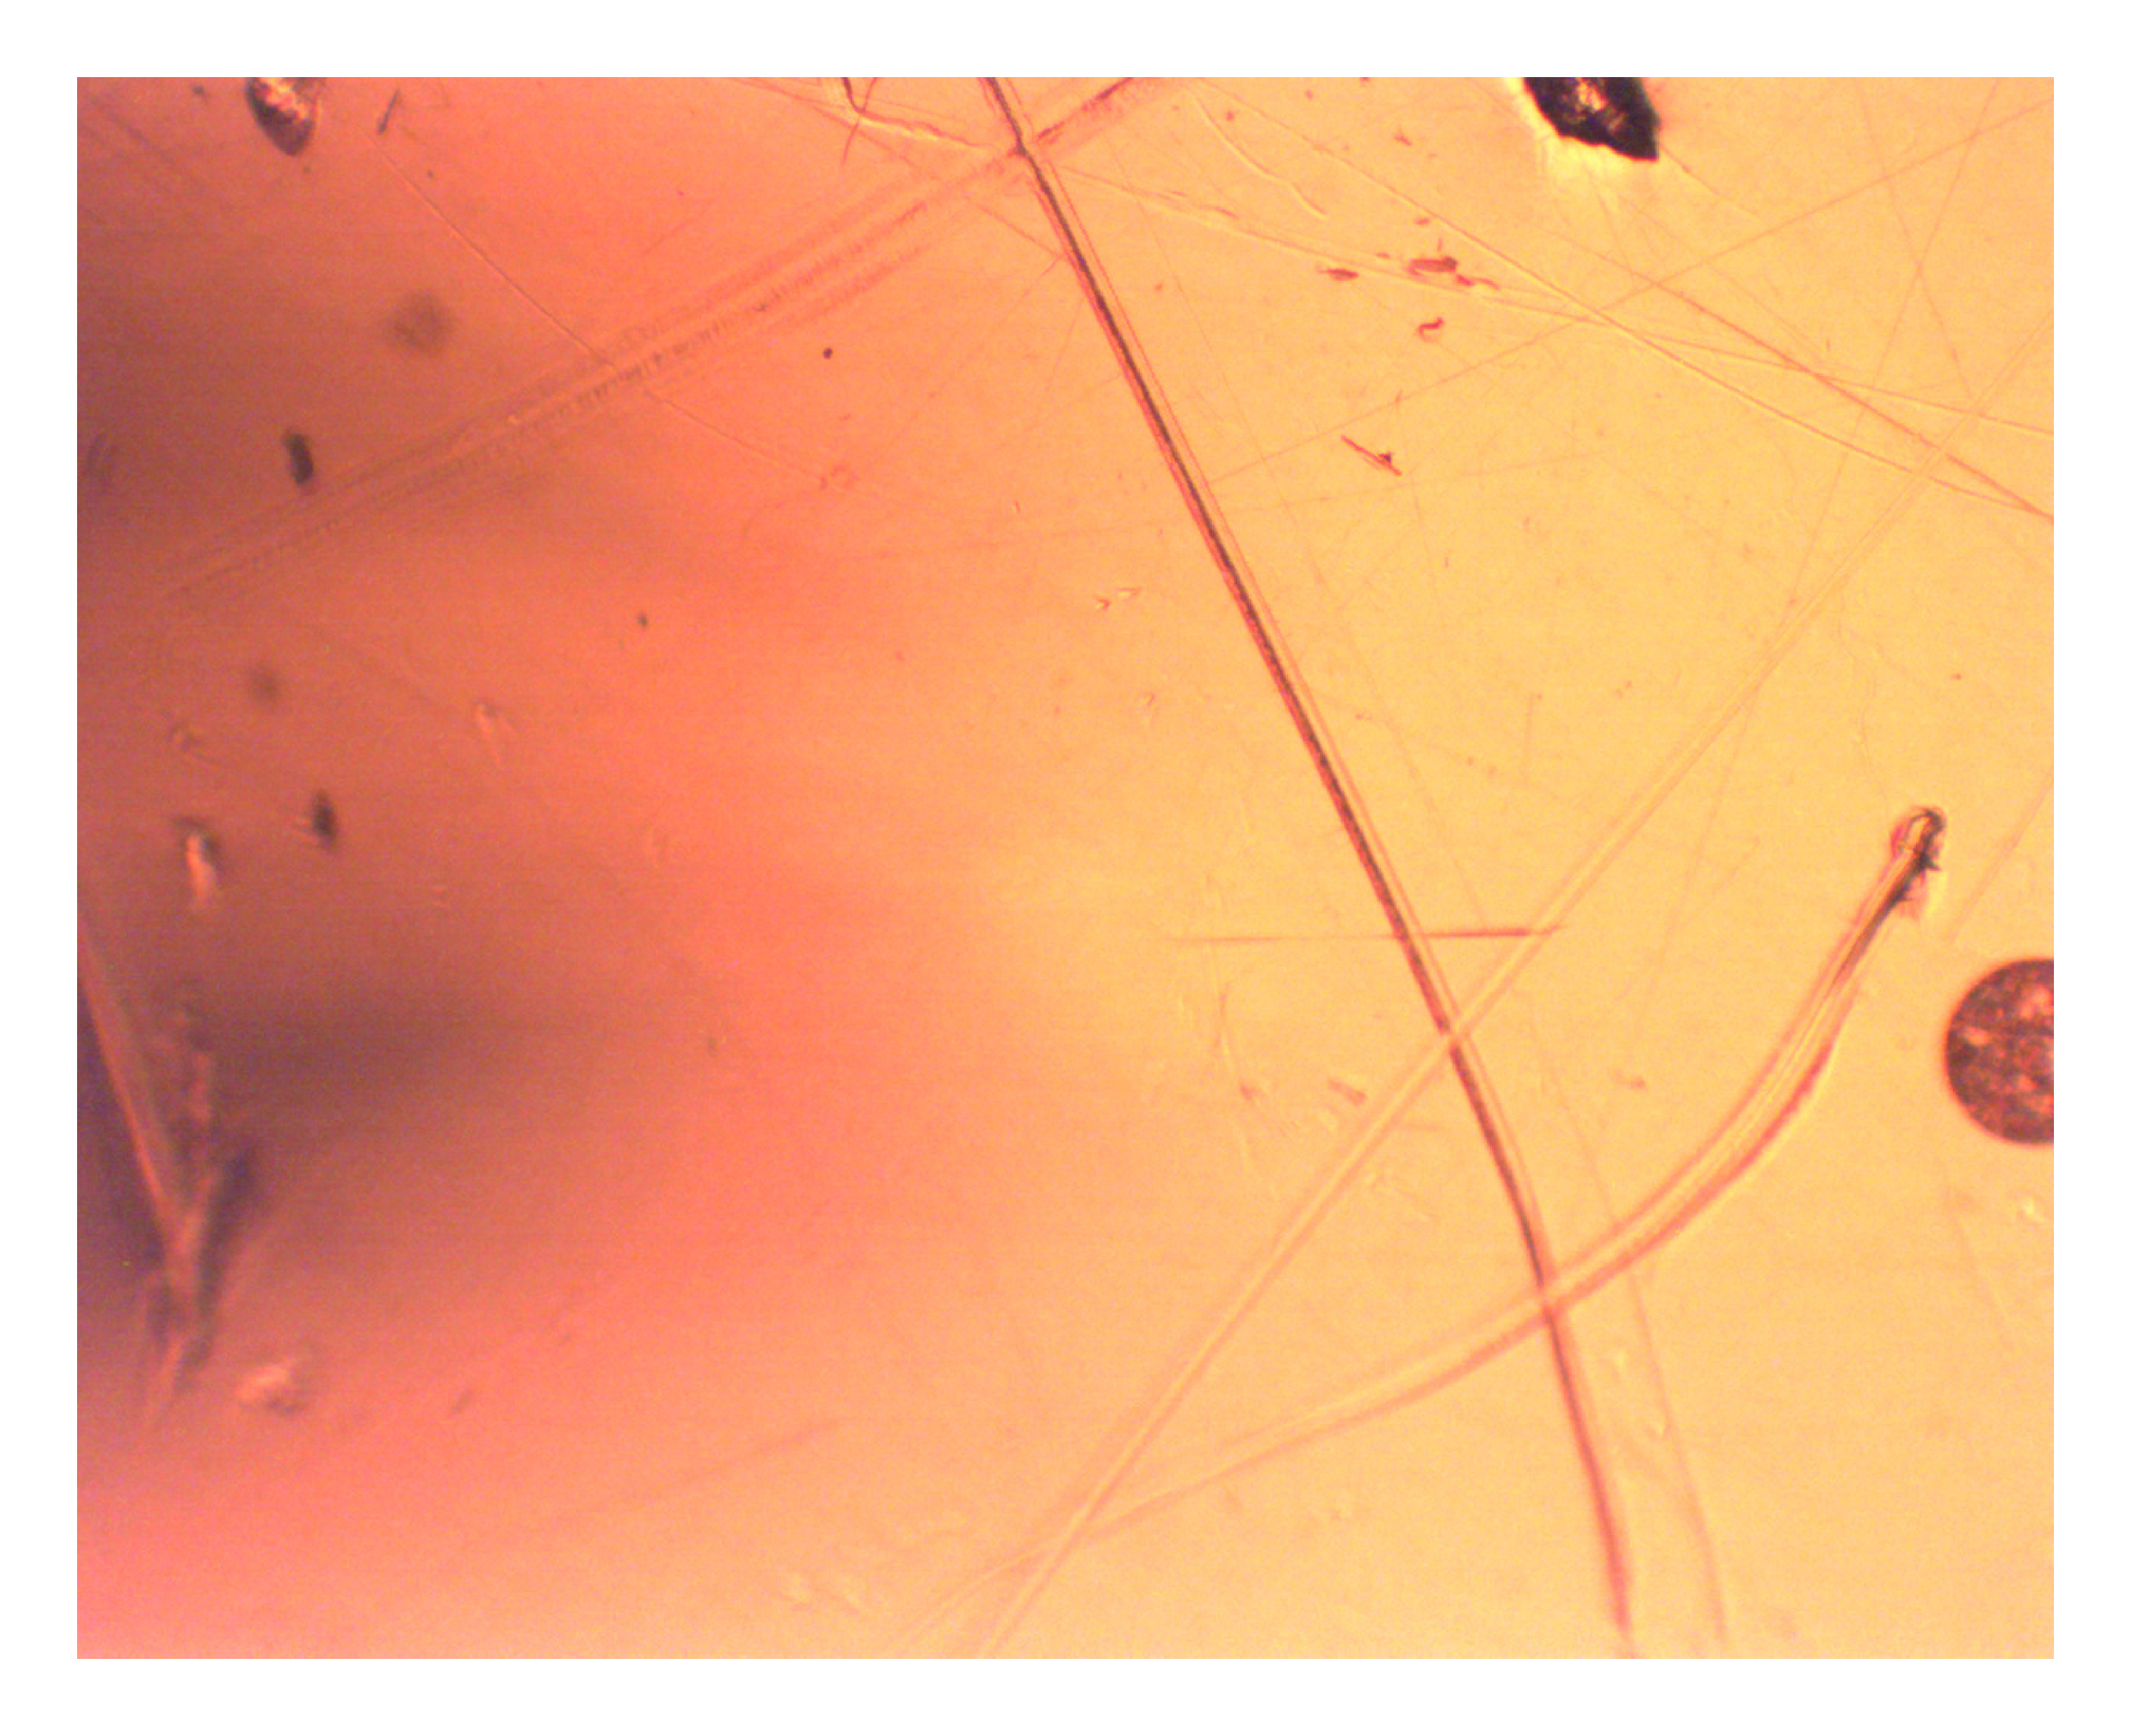
\includegraphics[width = 1\textwidth]{figures/chap4/CdTe_Ag_Zona2_10X.pdf}
        \subcaption{Zona 2 donde se realizo la medición de AFM y NSOM.}
    \end{subfigure}
\caption{Imágenes de las zonas de la muestra $ CdTe(001)/Ag $ estudiadas en AFM y NSOM.}
\label{fig:afm-zones}
\end{figure}

Podemos observar que las muestras tienen gran cantidad de ralladuras y detalles, los cuales 
pueden influir de manera negativa a la hora de calcular la rugosidad de la zona. Primero analizaremos 
la Zona 1, tomando algunos perfiles de linea para comparar su rugosidad con su respuesta óptica.

\subsubsection{Zona 1}
\label[type]{ch4:zone_1}

En esta zona, podemos observar en la Figura \ref{fig:afm-nsom-results}, que aunque la escala en
(a) muestra una variación de 0 a 55.6 nm, en (c) no presenta una gran variación en su rugosidad, 
siendo este gran intervalo ocasionado por las ralladuras presentes en la muestra.

Si comparamos (c) y (d), que están en el mismo perfil, vemos que aunque no exista una variación 
importante en la altura de la superficie, si existe un cambio en la respuesta óptica del 
material, esto solo puede deberse a que en esa zona, el índice de refracción varié porque la 
morfología es diferente.

Este fenómeno se puede apreciar mejor si observamos la respuesta de NSOM y AFM de forma 
tridimensional, como se aprecia en la Figura \ref{fig:afm-nsom-results-3d}, en donde podemos distinguir que en zonas planas 
vemos clústeres o islas en la respuesta óptica del material.

\begin{figure}[h!]
    \centering
    \begin{subfigure}[b]{0.45\textwidth}
        \centering
        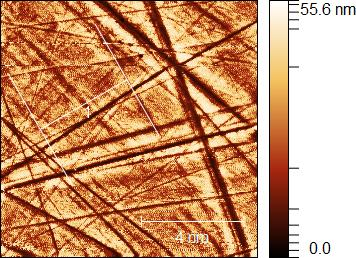
\includegraphics[width = 0.9\textwidth]{figures/chap4/CdTe_Ag_10um_256px_med1-Height_R.jpg}
        \subcaption{Resultados AFM de la zona de interés, en un área de 100 $n m^2$}
    \end{subfigure}\hfill
    \begin{subfigure}[b]{0.45\textwidth}
        \centering
        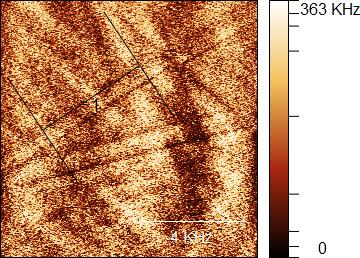
\includegraphics[width = 0.9\textwidth]{figures/chap4/CdTe_Ag_10um_256px_med1-NSOM_R}
        \subcaption{Resultados NSOM de la zona de interés, en un área de 100 $n m^2$ }
    \end{subfigure}

    \begin{subfigure}[b]{0.45\textwidth}
        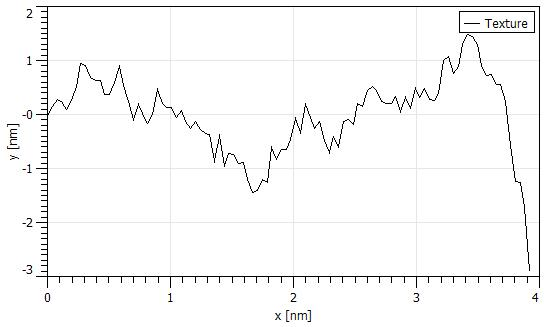
\includegraphics[width = 1\textwidth]{figures/chap4/CdTe_Ag_10um}
        \subcaption{Medición de la superficie sobre una linea en AFM, para observar la rugosidad de la superficie. }
    \end{subfigure}\hfill
    \begin{subfigure}[b]{0.45\textwidth}
        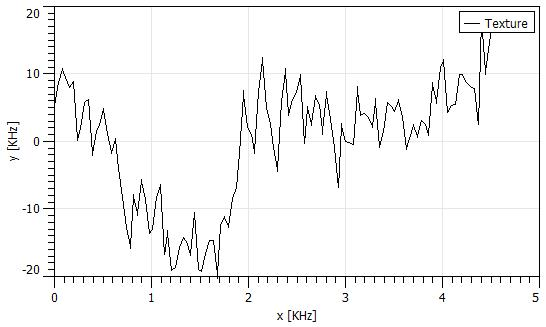
\includegraphics[width = 1\textwidth]{figures/chap4/CdTe_Ag_10um-nsom.jpg}
        \subcaption{Medición de la superficie sobre una linea en AFM, para observar los cambios del índice de refracción de la superficie.}
    \end{subfigure}

\caption{Resultados de la medición para la Zona 1.}
\label{fig:afm-nsom-results}
\end{figure}

\begin{figure}[h!]
    \centering
    \begin{subfigure}[b]{0.5\textwidth}
        \centering
        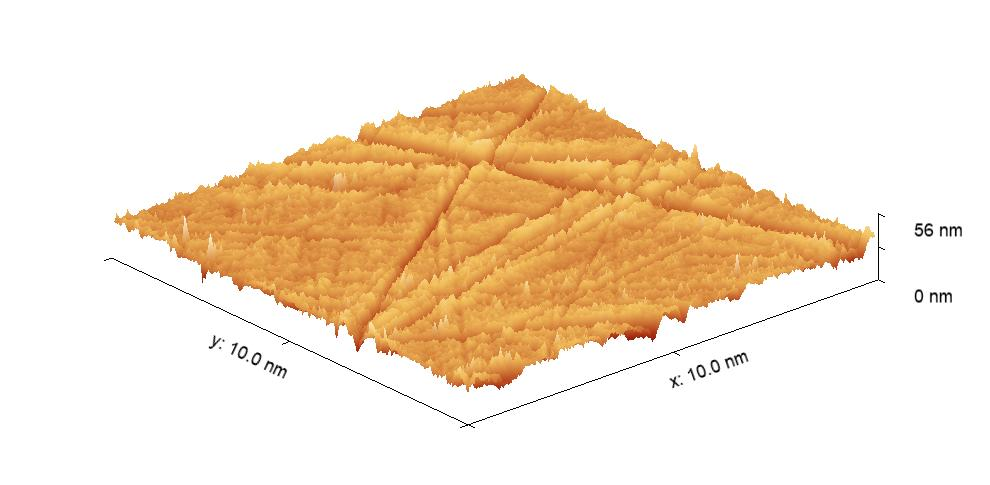
\includegraphics[width = 1\textwidth]{figures/chap4/CdTe_Ag_10um-3d.jpg}
        \subcaption{Resultados AFM de la zona de interés, en un área de 100 $n m^2$}
    \end{subfigure}\hfill
    \begin{subfigure}[b]{0.5\textwidth}
        \centering
        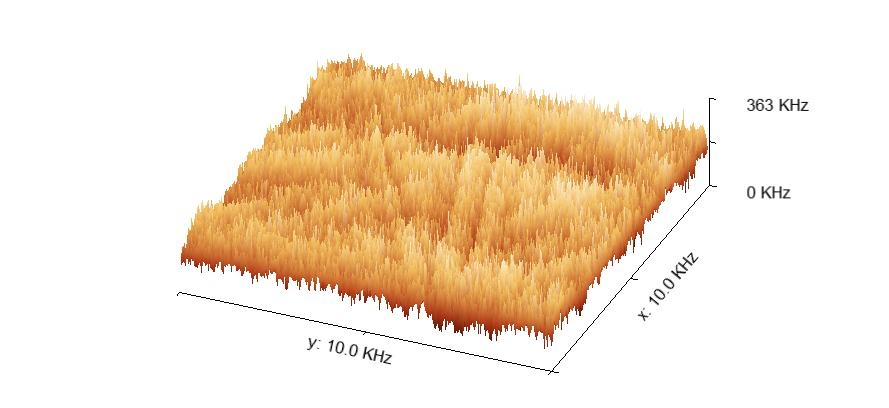
\includegraphics[width = 1\textwidth]{figures/chap4/CdTe_Ag_10um-3d-nsom.jpg}
        \subcaption{Resultados NSOM de la zona de interés, en un área de 100 $n m^2$ }
    \end{subfigure}

\caption{Representación tridimensional para las mediciones de AFM y NSOM de la Zona 1.}
\label{fig:afm-nsom-results-3d}
\end{figure}
\newpage

\section{Experimentos sobre $ Hg_{0.18}Cd_{0.82}Te (001)$}
\label{sec:chap4-hgcdte}
En esta sección se discuten los espectros de \textit{RDS} realizados sobre una muestra de $ Hg_{0.18}Cd_{0.82}Te (001)$ 
sin y con daño superficial y sus espectros de la Espectroscopia Raman. Como se ha mencionado el 
$ Hg_{0.18}Cd_{0.82}Te (001)$ es un material semimetálico y su brecha fundamental es muy pequeña. Una de las formas para 
romper la degeneración de la brecha fundamental es reduciendo la dimensionalidad del material, ya sea en estructuras de 
pozos o puntos cuánticos o aplicando una tensión. Esta tensión puede ser aplicada externamente por medio de un esfuerzo 
mecánico o generando defectos superficiales, como las dislocaciones.

En el último caso, la tensión estará localizada en los primeros micrómetros por debajo de la superficie. De esta forma 
la superficie pierde su carácter semimetálico, mientras que el bulto seguirá siendo un semimetal. La idea fundamental de 
estos experimentos es identificar los compontes de la \textit{RDS} inducidas por la tensión superficial y diferenciarlos 
de los inducidos por una superficie semimetálica.


\subsection{\textit{RDS} sobre superficies talladas mecánicamente}
\label{sec:chap4-hgcdte-rds}
Con el objeto de romper la degeneración de las bandas de energía en el punto $\Gamma$ y abrir la brecha fundamental del 
Cd0.18Hg0.82Te, se realizó un ligero tallado superficial con abrasivo de diamante de tamaño de grano de $ 0.25 \mu m $ 
a lo largo de la dirección [110]. Es bien sabido que este procedimiento genera defectos lineales paralelos a la 
superficie y por tanto un campo de tensión cercano a la superficie que se extiende algunas micras hacia su interior\cite{LastrasMartnez1996}. L
a tensión cambia la simetría del cristal y por tanto rompe la degeneración de los niveles. 

\begin{figure}[h!]
    \centering
    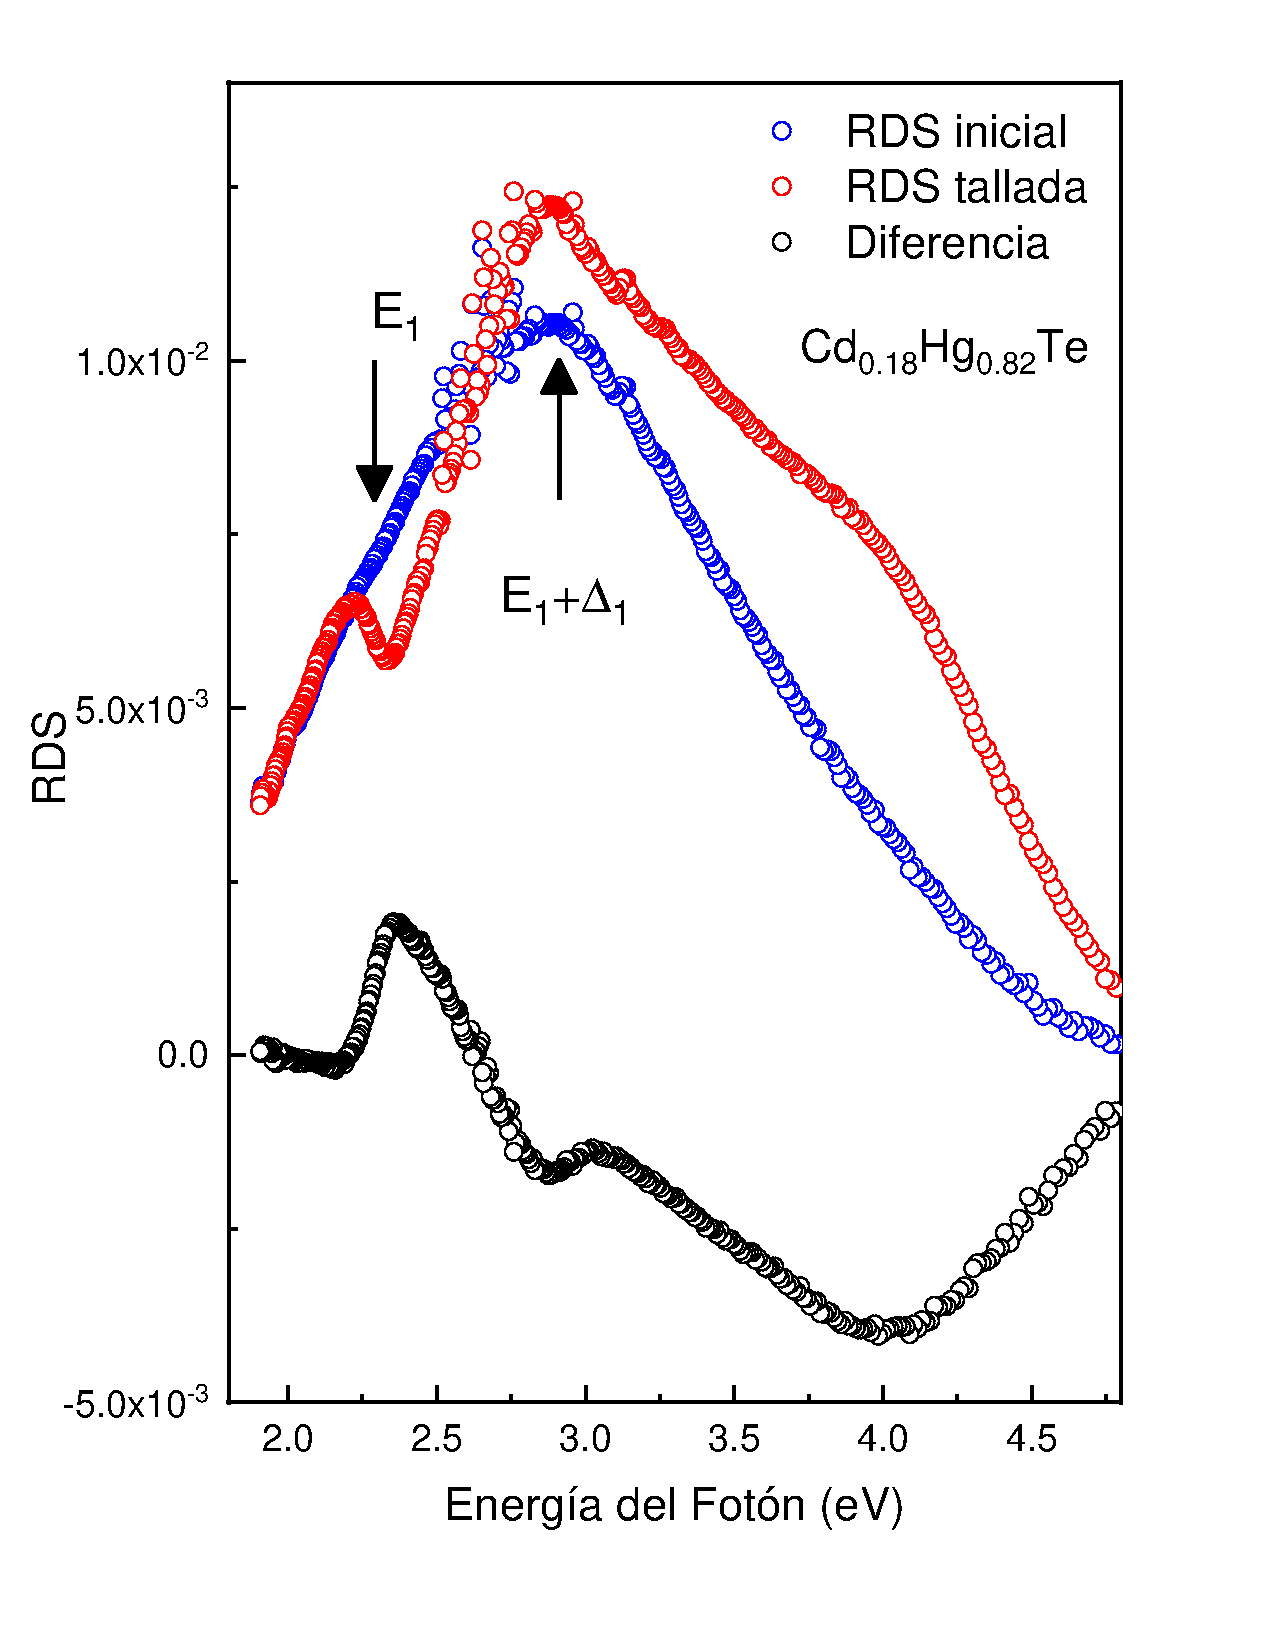
\includegraphics[width=0.7\textwidth]{figures/chap4/hgcdte_rds_comparision.pdf}
        \caption{Espectros \textit{RDS} obtenidos para $ Hg_{0.18}Cd_{0.82}Te (001)$ \textit{(azul)} y 
        $ Hg_{0.18}Cd_{0.82}Te (001)$ tallado mecánicamente \textit{(rojo)}, además de observar la diferencia entre 
        ambos \textit{(negro)}.}
    \label{fig:hgcdte_rds_comparision}
\end{figure}

De esta forma, se tiene una superficie menos metálica respecto al bulto del material. En la 
\ref{fig:hgcdte_rds_comparision} se presentan los resultados experimentales de RDS obtenidos para la muestra sin 
tallado superficial (puntos azules), con tallado (puntos rojos) y la diferencia numérica entre ambos (puntos negros) 
en el rango espectral de 2.0-4.5 eV. 
Este rango corresponde a las transiciones $E_{1}$ y $E_{1}+\Delta1$ del Cd0.18Hg0.82Te\cite{Camacho2005}. Obsérvese que 
el espectro sin tallar es suave y no tiene estructuras evidentes alrededor de $E_{1}$ y $E_{1}+\Delta1$. Esto puede 
estar relacionado al carácter metálico del Cd0.18Hg0.82Te que apantalla la contribución de las transiciones 
$E_{1}$ y $E_{1}+\Delta1$ al espectro de RDS. 

Al tallar la muestra se genera un incremento en la anisotropía y se rompe la degeneración del punto $\Gamma$. El 
espectro de puntos rojos en la Figura \ref{fig:hgcdte_rds_comparision} corresponde a la muestra tallada. Obsérvese 
como se incrementa notablemente la estructura alrededor de   las transiciones $E_{1}$ y $E_{1}+\Delta1$. Para asilar 
la componente inducida por el tallado en la RDS, se muestra el espectro obtenido restando numéricamente los espectros 
rojo y azul. Este resultado se muestra en el espectro negro. En este último, las estructuras de las transiciones 
$E_{1}$ y $E_{1}+\Delta1$ son muy evidentes.

\subsubsection{Análisis de la tensión superficial}
\label{sec:chap4-hgcdte-rds-stress}
Con el objetivo de cuantificar la tensión promedio en la superficie inducida por el tallado, 
se realizó un ajuste al modelo de tensión en \textit{RDS}. La forma de línea de RD bajo tensión \textit{X}, está dada 
por\cite{LastrasMartnez2010}:

\begin{equation}
    \frac{\Delta R}{R} = Re [\frac{1}{r n}\frac{\partial r}{\partial E} (df_{1} + df_{2})]
\end{equation}

Donde \textit{n} es el índice complejo de refracción del material (la función dieléctrica está dada por 
$ \epsilon = n^{2}$ ) y $ r=\frac{1-n}{n+1} $ es la reflexión a incidencia normal. 
Los factores $df_{1}$ y $df_{2}$ están dados por:

\begin{equation}
    df_{1} = \frac{4\gamma}{\Delta_{1}} \epsilon^{(1)} +  \Delta E_{s}\frac{\partial \epsilon^{(1)}}{\partial E}
\end{equation}

\begin{equation}
    df_{2} = {-\frac{4\gamma}{\Delta_{1}} \epsilon^{(2)}} +  \Delta E_{s}\frac{\partial \epsilon^{(2)}}{\partial E} 
\end{equation}

Siendo $\epsilon^{(1)}$ y $\epsilon^{(2)}$ son las contribuciones a la función dieléctrica compleja de los puntos 
$E_{1}$ y $E_{1}+\Delta1$ respectivamente, $\gamma = \frac{S_{44} D_{3}^{5} X}{2\sqrt{6}}$ y 
$\Delta E_{s} = \frac{S_{44} D_{1}^{5} X}{4\sqrt{3}}$. 
El parámetro  $S_{44}$ es el módulo elástico de compliancia (\textit{elastic compliance moduli}) y $D_{1}^{5}$ y 
$D_{3}^{5}$ son los potenciales de deformación.

Para realizar el cálculo de la forma de línea del espectro de RDS, se ajustaron con curvas Lorenzianas las formas de línea de 
las funciones dieléctricas de Cd0.18Hg0.82Te obtenidas por medio de elipsometria\cite{Camacho2005}. Las formas de línea 
y los parámetros utilizados para ajustar la RDS se muestran en la Tabla ? y Tabla ? 
respectivamente\cite{LastrasMartnez2009}\cite{LastrasMartnez2010}. 

La Fig. \ref{fig:hgcdte_rds_stress} se muestra la contribución de la tensión superficial al espectro de RDS y el 
ajuste obtenido con el modelo y los parámetros de las Tablas ? y ?. Obsérvese como el modelo describe excelentemente 
la forma de línea reafirmando el origen de tensión de la \textit{RDS}. Del ajuste se encuentra que el valor medio 
de $ X = -0.24x10^{9} \frac{dyn}{cm^{2}}$.

\begin{figure}[h!]
    \centering
    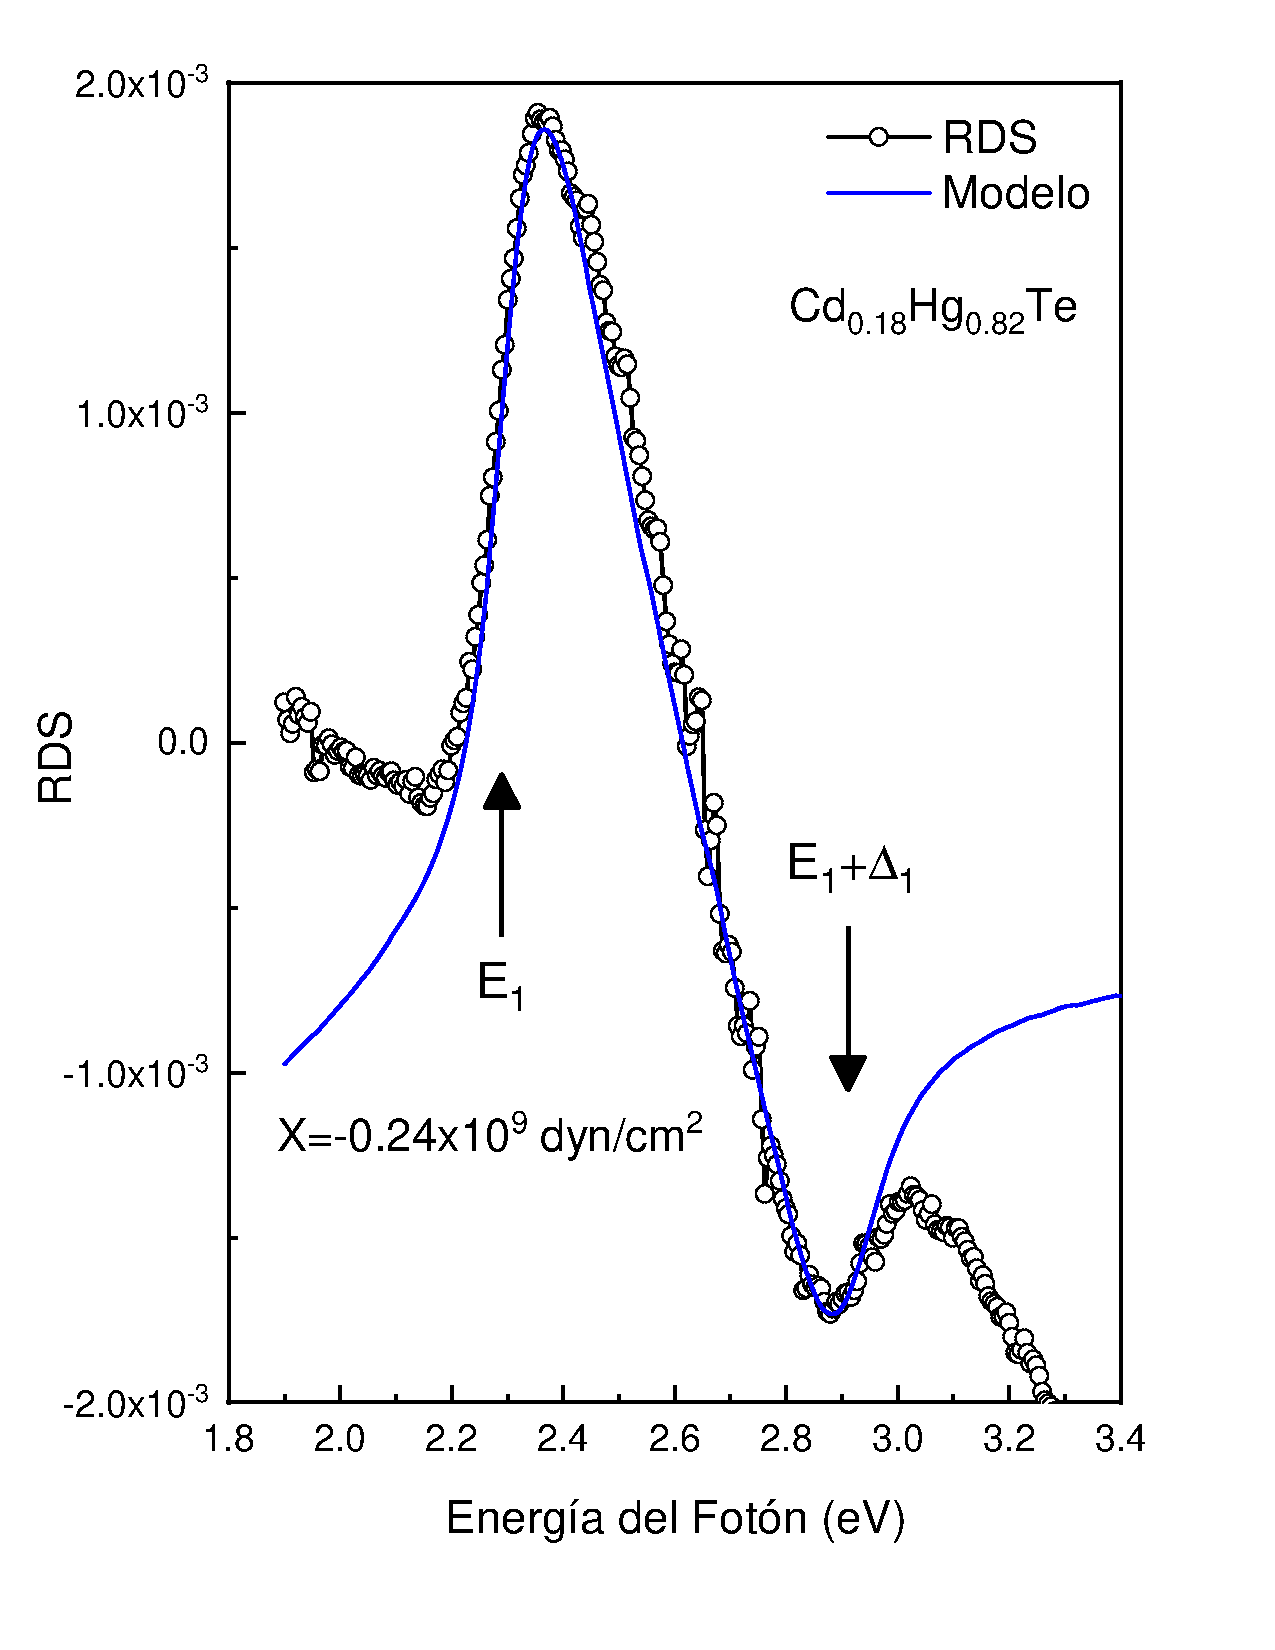
\includegraphics[width=0.7\textwidth]{figures/chap4/hgcdte_rds_stress.pdf}
        \caption{Espectros \textit{RDS} obtenidos para $ Hg_{0.18}Cd_{0.82}Te (001)$ modelado \textit{(azul)} y 
        $ Hg_{0.18}Cd_{0.82}Te (001)$ tallado mecánicamente \textit{(negro)}, para obtener el calculo del estrés
        promedio \textit{X}.}
    \label{fig:hgcdte_rds_stress}
\end{figure}


Este valor esta en el orden de magnitud de los típicos valores de tensión mecánica externa aplicados en experimentos 
de materiales como el $ CdTe $ \cite{LastrasMartnez2010}. De esta forma, podemos establecer que la técnica de RDS nos 
permite distinguir entre el carácter semimetálico del material y el producido por un rompimiento de simetría,
como el de los defectos lineales generados. Este resultado es importante, ya que abre la posibilidad de contar con una 
herramienta óptica para la caracterización de superficies de CdHgTe bajo tensión o interfaces de CdTe/CdHgTe dentro de 
una estructura de pozos con carácter de aislante topológico.
\newpage

\subsection{Espectroscopia Raman sobre superficies talladas mecánicamente}
\label{sec:chap4-hgcdte-raman}

Se obtuvo los siguientes espectros Raman para HgCdTe(001) y HgCdTe(001) tallado mecánicamente.
\begin{figure}[h!]
    \centering
    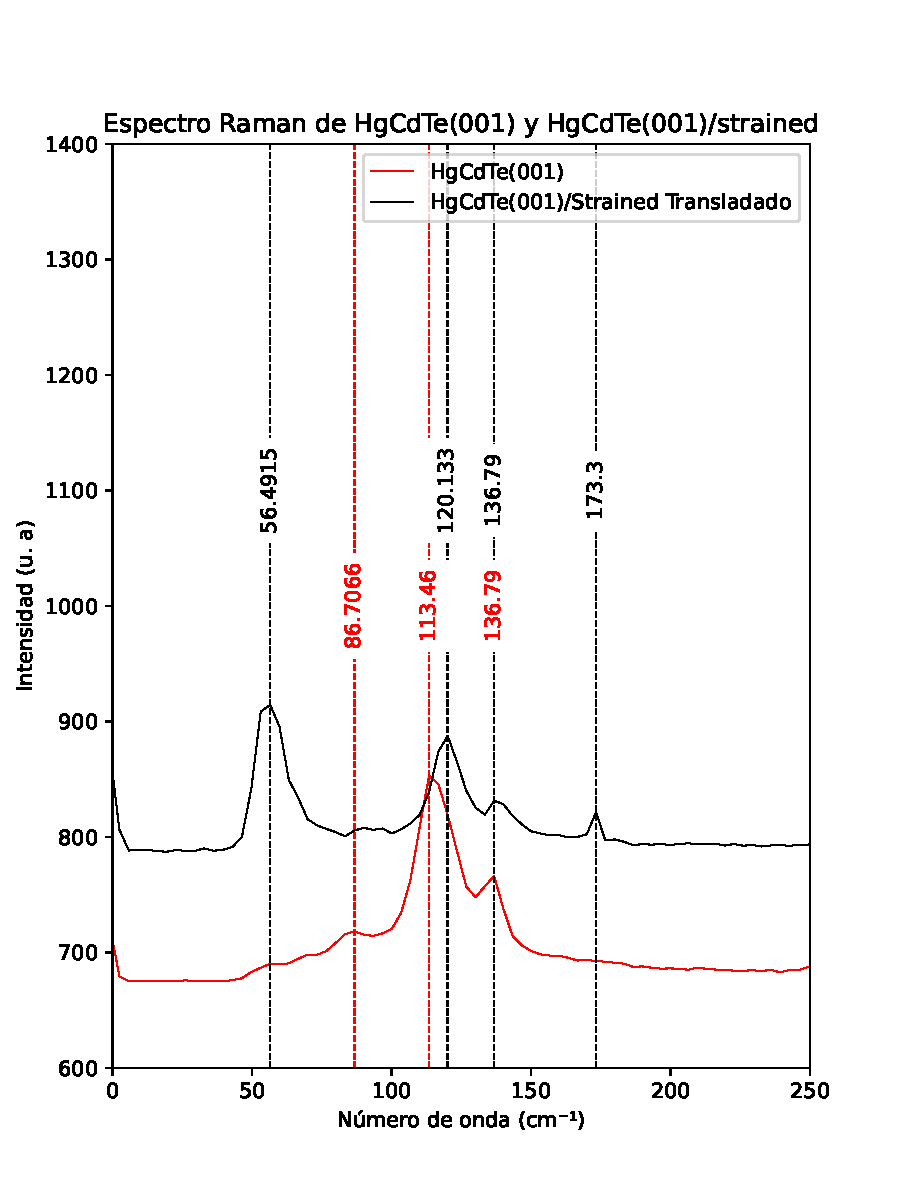
\includegraphics[width=0.7\textwidth]{figures/chap4/raman-HgCdTes-250-T.pdf}
        \caption{Espectros Raman obtenidos para $ Hg_{0.18}Cd_{0.82}Te (001)$ y 
        $ Hg_{0.18}Cd_{0.82}Te (001)$ tallado mecánicamente.}
    \label{fig:hgcdte_rds_stress}
\end{figure}

En la Figura \ref{fig:hgcdte_rds_comparision}, podemos observar que al contrario del sistema 
CdTe(001)/Ag, donde la tensión solo parecía afectar la posición de los picos, su altura relativa 
y su FWHM, aqui cambia totalmente \textit{la simetría} de la superficie, obteniendo dos estructuras 
mas en 56.4915 y 173.3 $cm^(-1)$. En la Tabla ?, podemos apreciar el cambio entre los semianchos 
de los picos que comparten ambos espectros.

Cabe destacar que al ser parte de la aleación HgCdTe, el CdTe comparte un pico en el espectro Raman 
que parece imperturbable a los cambios que se someta en su superficie, aunque su Samanco si varié.
***Checar paper nuevo, significado To y Lo cada peak*** 
